\documentclass[leqno,usenames,dvipsnames,14pt]{beamer}
\usetheme{Singapore}
\usepackage{xcolor}
\usepackage{amsmath}
\usepackage{graphicx}
\title{Solving Problems Using Linear Equations}
\author{}
\date{}

\begin{document}


% Slide 1: Introduction
\begin{frame}
    \titlepage
\end{frame}

% Slide 2: Example 1 Question
\begin{frame}{Example 1: Linear Equation Problem}
\Large
  When five times a certain number is reduced by 4, the result is the same as adding 7 to four times the number. Find the number.
\end{frame}

% Slide 3: Example 2 Question
\begin{frame}{Example 2: Rectangle Perimeter}
    \textbf{Question:} (i) Find an expression, in terms of \( x \), for the perimeter of this rectangle.\\
    (ii) The perimeter of the rectangle is 44 cm. Write down an equation and solve it to find the value of \( x \).
    
    \begin{center}
        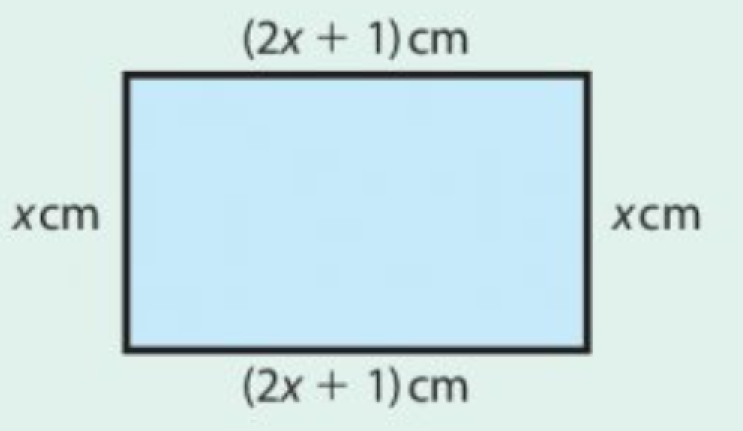
\includegraphics[width=0.5\textwidth]{images/alg001.png}
    \end{center}
\end{frame}

\begin{frame}
\end{frame}








% Slide 4: Exercise 1.5, Question 1
\begin{frame}{Exercise 1.5, Question 1}
\Large
  If I multiply a number by 4 and then add 3, the result is the same as adding 8 to three times the number. Form an equation in \( x \) and solve it to find the number.
\end{frame}

% Slide 5: Exercise 1.5, Question 2
\begin{frame}{Exercise 1.5, Question 2}
\Large
  I think of a number, multiply it by 8 and then subtract 2. I get the same result as when I multiply this number by 2 and add 10. What is this number?
\end{frame}

% Slide 6: Exercise 1.5, Question 3
\begin{frame}{Exercise 1.5, Question 3}
\Large
  One number is 5 greater than another number. If the smaller number is added to twice the larger number, the answer is 28. Find the two numbers.
\end{frame}

% Slide 7: Exercise 1.5, Question 4
\begin{frame}{Exercise 1.5, Question 4}
\Large
  Ann is 3 years older than Helen. If twice the sum of their ages is 50 years, how old is Ann?
\end{frame}

% Slide 8: Exercise 1.5, Question 5
\begin{frame}{Exercise 1.5, Question 5}
\Large
  (i) Find an expression for the perimeter of this triangle.\\
  (ii) What value of \( x \) gives a perimeter of 55?

  \begin{center}
    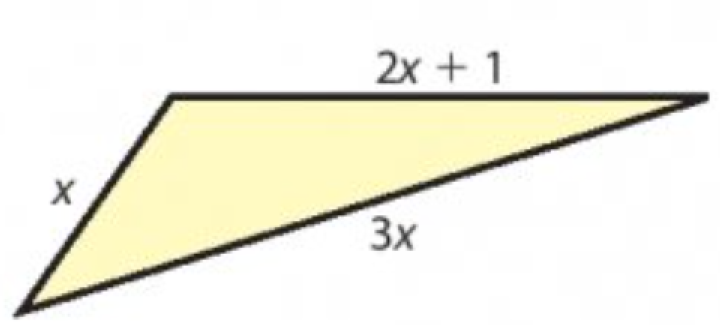
\includegraphics[width=0.5\textwidth]{images/alg002.png}
  \end{center}
\end{frame}

% Slide 9: Exercise 1.5, Question 6
\begin{frame}{Exercise 1.5, Question 6}
\Large
  If we subtract 4 from a number and then multiply the result by 5, the answer is 15. Find the number.
\end{frame}

% Slide 10: Exercise 1.5, Question 7
\begin{frame}{Exercise 1.5, Question 7}
\Large
  I think of a number, increase it by 4 and double the answer. The result is 20 more than the number. Find this number.
\end{frame}

% Slide 11: Exercise 1.5, Question 8
\begin{frame}{Exercise 1.5, Question 8}
\Large
  Use your knowledge of angles to form an equation and solve it to find the value of \( a \).

  \begin{center}
    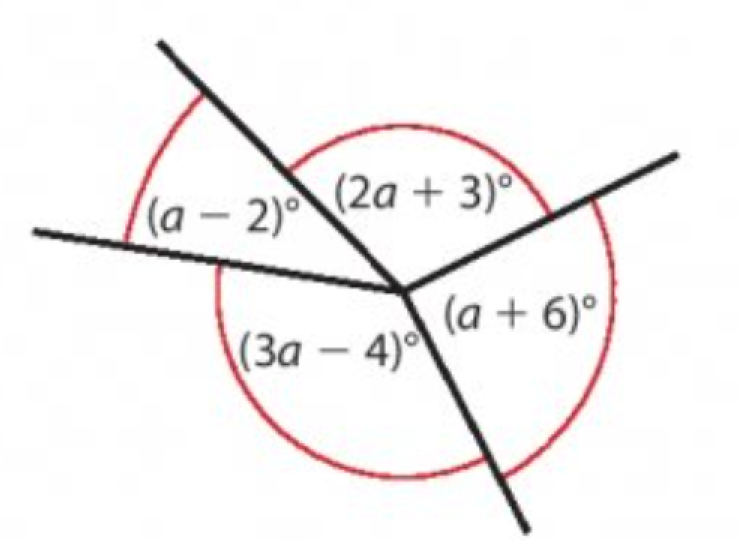
\includegraphics[width=0.5\textwidth]{images/alg003.png}
  \end{center}
\end{frame}

% Slide 12: Exercise 1.5, Question 9
\begin{frame}{Exercise 1.5, Question 9}
\Large
  A triangle and rectangle are shown below:

  \begin{center}
    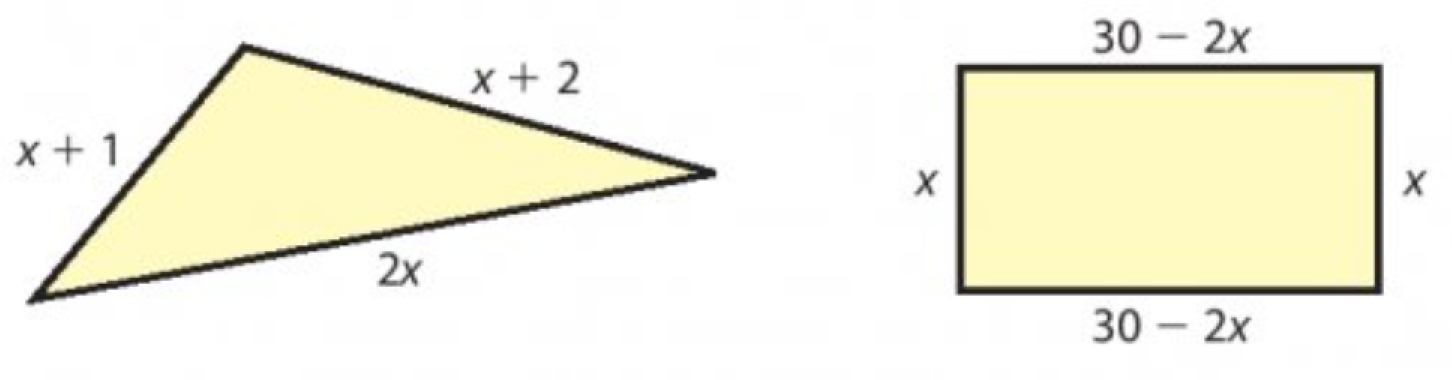
\includegraphics[width=0.5\textwidth]{images/alg004.png}
  \end{center}
  
  Find the value of \( x \) which:
  \begin{enumerate}
    \item gives a triangle with a perimeter of 63.
    \item gives a triangle and rectangle with equal perimeters.
    \item makes the rectangle into a square.
  \end{enumerate}
\end{frame}

% Slide 13: Exercise 1.5, Question 10
\begin{frame}{Exercise 1.5, Question 10}
\Large
  The sum of three consecutive odd numbers is 57. Find these numbers.
\end{frame}

% Slide 14: Exercise 1.5, Question 11
\begin{frame}{Exercise 1.5, Question 11}
\Large
  Two opposite angles in a parallelogram are \( (2x + 5)^\circ \) and \( (3x - 35)^\circ \). Find the value of \( x \).

  \begin{center}
    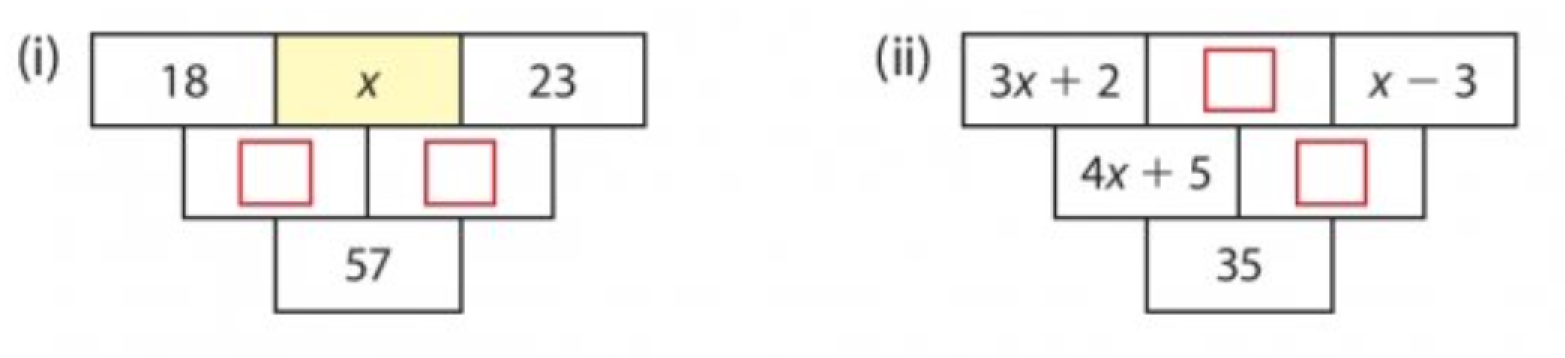
\includegraphics[width=0.5\textwidth]{images/alg005.png}
  \end{center}
\end{frame}

% Slide 15: Exercise 1.5, Question 12
\begin{frame}{Exercise 1.5, Question 12}
\Large
  A straight line intersects a triangle forming three angles \( (x - 10)^\circ, (2x + 20)^\circ \), and \( (3x - 30)^\circ \). Find the value of \( x \).

  \begin{center}
    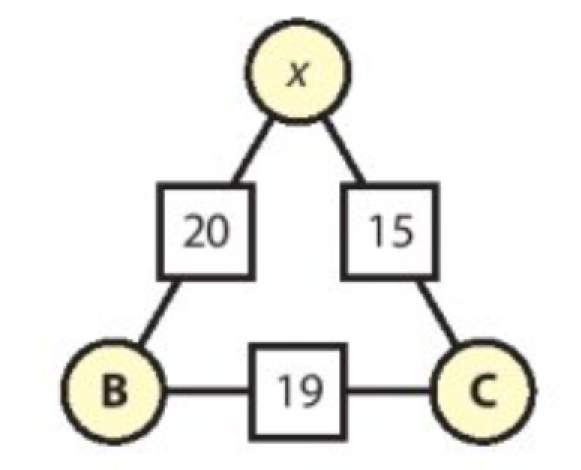
\includegraphics[width=0.5\textwidth]{images/alg006.png}
  \end{center}
\end{frame}

% Slide 16: Exercise 1.5, Question 13
\begin{frame}{Exercise 1.5, Question 13}
\Large
  Find three consecutive numbers such that the square of the smallest number is 5 more than the square of the largest number.

  \begin{center}
    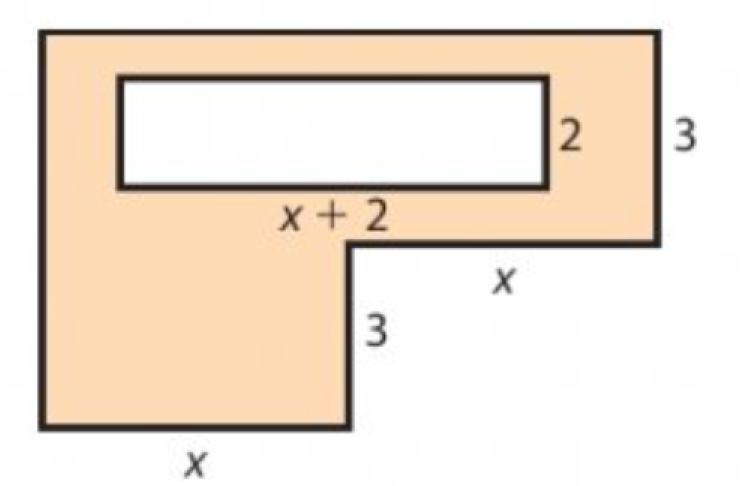
\includegraphics[width=0.5\textwidth]{images/alg007.png}
  \end{center}
\end{frame}

% Slide 17: Exercise 1.5, Question 14
\begin{frame}{Exercise 1.5, Question 14}
\Large
  Find the value of \( x \) if the sum of \( 4x + 7 \) and \( 3x - 2 \) is equal to 29.
\end{frame}

% Slide 18: Exercise 1.5, Question 15
\begin{frame}{Exercise 1.5, Question 15}
\Large
  The difference between twice a number and 4 is equal to 3 times the number less 7. Find the number.
\end{frame}












\end{document}
